		
	\section{Introduction}
	L’objectif de ce projet est de déployer un serveur \textbf{DHCP (Dynamic Host Configuration Protocol)}, chargé d’attribuer automatiquement des adresses IP aux clients d’un réseau, ainsi qu’un pare-feu configuré avec \texttt{iptables} pour sécuriser les connexions entrantes. Le tout sera mis en place sur un système Debian installé dans une machine virtuelle via \texttt{VirtualBox}. L’installation et la configuration de ces services seront automatisées à l’aide d’un script Bash. Enfin, une image Docker du système configuré sera créée pour faciliter son déploiement dans d’autres environnements.
	
	\section{Prérequis et outils utilisés}
	\begin{itemize}
		\item Système d’exploitation : Debian 12
		\item Docker et ses dépendances
		\item iptables / iptables-persistent
		\item isc-dhcp-server
		\item Droits administrateur (root)
	\end{itemize}
	
	\section{Description du script automatisé}
	
	Le script Bash \texttt{setup-dhcp-firewall.sh} permet d’automatiser l’ensemble du processus de création d’un serveur DHCP sécurisé dans un conteneur Docker.
	
	\subsection*{Étape 1 : Collecte des paramètres réseau}
	L'utilisateur saisit les informations nécessaires à la configuration du DHCP :
	\begin{itemize}
		\item Adresse réseau
		\item Masque de sous-réseau
		\item Plage IP
		\item Passerelle
		\item Serveur DNS
	\end{itemize}
	
	\begin{lstlisting}
		echo "[1/8] Demande des informations de configuration réseau pour le DHCP..."
		read -p "Adresse réseau (ex: 192.168.100.0): " RESEAU
		read -p "Masque de sous-réseau (ex: 255.255.255.0): " NETMASK
		read -p "Adresse IP de début (ex: 192.168.100.100): " IP_DEBUT
		read -p "Adresse IP de fin (ex: 192.168.100.200): " IP_FIN
		read -p "Passerelle (ex: 192.168.100.1): " GATEWAY
		read -p "DNS (ex: 8.8.8.8): " DNS
	\end{lstlisting}
	
	\subsection*{Étape 2 : Installation de Docker}
	\begin{lstlisting}
		echo "[2/8] Mise à jour du système et installation de Docker..."
		apt update && apt upgrade -y
		apt install -y ca-certificates curl gnupg lsb-release
		
		install -m 0755 -d /etc/apt/keyrings
		curl -fsSL https://download.docker.com/linux/debian/gpg -o /etc/apt/keyrings/docker.asc
		chmod a+r /etc/apt/keyrings/docker.asc
		
		echo "deb [arch=$(dpkg --print-architecture) signed-by=/etc/apt/keyrings/docker.asc] https://download.docker.com/linux/debian $(. /etc/os-release && echo "$VERSION_CODENAME") stable" | tee /etc/apt/sources.list.d/docker.list > /dev/null
		
		apt update
		apt install -y docker-ce docker-ce-cli containerd.io docker-buildx-plugin docker-compose-plugin
	\end{lstlisting}
	
	\subsection*{Étape 3 : Nettoyage des ressources existantes}
	\begin{lstlisting}
		echo "[3/8] Nettoyage des anciens fichiers (si présents)..."
		rm -rf docker-firewall
		docker rm -f mon-serveur-dhcp 2>/dev/null || true
		docker image rm dhcp-firewall 2>/dev/null || true
	\end{lstlisting}
	
	\subsection*{Étape 4 : Création de l’environnement Docker}
	\begin{lstlisting}
		echo "[4/8] Création des fichiers Docker..."
		mkdir -p docker-firewall
		cd docker-firewall
	\end{lstlisting}
	
	\textbf{Contenu de script-firewall.sh :}
	\begin{lstlisting}
		#!/bin/bash
		iptables -F
		iptables -X
		iptables -P INPUT DROP
		iptables -P FORWARD DROP
		iptables -P OUTPUT ACCEPT
		iptables -A INPUT -i lo -j ACCEPT
		iptables -A INPUT -m conntrack --ctstate ESTABLISHED,RELATED -j ACCEPT
		iptables -A INPUT -p icmp --icmp-type 8 -j DROP
		netfilter-persistent save
	\end{lstlisting}
	
	\textbf{Contenu de script-dhcp.sh :}
	\begin{lstlisting}
		#!/bin/bash
		echo 'DHCPDv4_CONF=/etc/dhcp/dhcpd.conf' > /etc/default/isc-dhcp-server
		echo 'INTERFACESv4="enp0s3"' >> /etc/default/isc-dhcp-server
		
		cat <<EOL > /etc/dhcp/dhcpd.conf
		option domain-name "gerioux.com";
		default-lease-time 345600;
		max-lease-time 691200;
		authoritative;
		log-facility local7;
		
		subnet $RESEAU netmask $NETMASK {
			range $IP_DEBUT $IP_FIN;
			option domain-name-servers $DNS;
			option routers $GATEWAY;
		}
		EOL
		
		systemctl restart isc-dhcp-server.service
	\end{lstlisting}
	
	\textbf{Contenu de Dockerfile :}
	\begin{lstlisting}
		FROM debian:stable-slim
		
		RUN apt update && apt install -y iptables iptables-persistent isc-dhcp-server net-tools nano systemctl
		
		COPY script-dhcp.sh /root/script-dhcp.sh
		COPY script-firewall.sh /root/script-firewall.sh
		
		RUN chmod +x /root/script-dhcp.sh /root/script-firewall.sh
		
		CMD /root/script-firewall.sh && /root/script-dhcp.sh && tail -f /dev/null
	\end{lstlisting}
	
	\subsection*{Étape 5 : Construction de l’image Docker}
	\begin{lstlisting}
		chmod +x script-dhcp.sh script-firewall.sh
		echo "[5/8] Construction de l’image Docker..."
		docker build -t dhcp-firewall .
	\end{lstlisting}
	
	\subsection*{Étape 6 : Lancement du conteneur}
	\begin{lstlisting}
		echo "[6/8] Lancement du conteneur DHCP + Pare-feu..."
		docker run --rm --net=host --cap-add=NET_ADMIN --name mon-serveur-dhcp dhcp-firewall
	\end{lstlisting}
	
	\section{Résultats et vérification}
	Après exécution, on vérifie que :
	\begin{itemize}
		\item Le serveur DHCP fonctionne et attribue des adresses IP
		\item Les règles de pare-feu bloquent les connexions non sollicitées
		\item Le conteneur reste actif et les services fonctionnent
	\end{itemize}

 \section{Création de l’instance sur AWS}

\vspace{1em}
 \subsection{Définition du nom de l’instance}
% TODO: \usepackage{graphicx} required
\begin{figure}[h!]
	\centering
	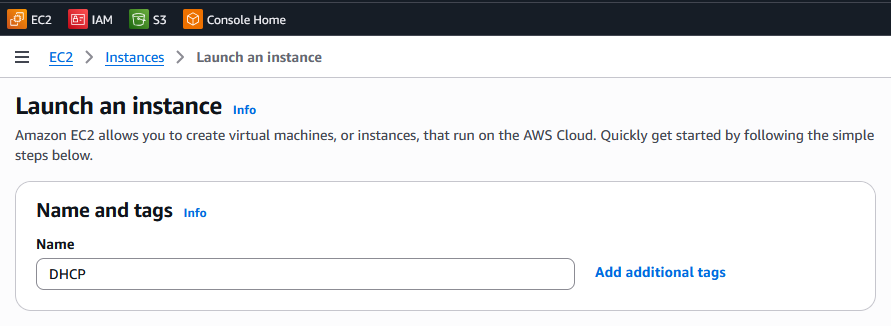
\includegraphics[width=0.8\linewidth]{corps/images/image1}
	%\caption{}
	\label{fig:1}
\end{figure}

\subsection{Choix du système d’exploitation}
	\begin{figure}[h!]
		\centering
		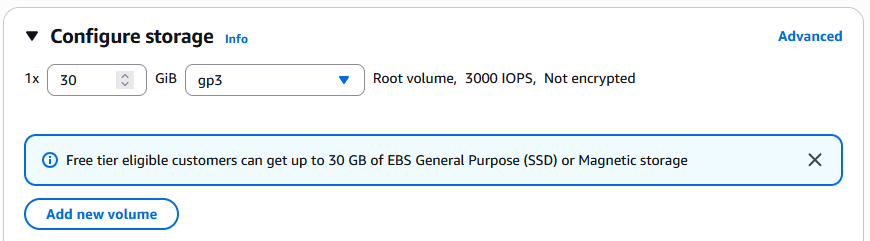
\includegraphics[width=0.8\linewidth]{corps/images/image2}
		%\caption{}
		\label{fig:2}
	\end{figure}

\subsection{Choix d’instance (Nous avons choisi la version gratuite)}
\begin{figure}[h!]
	\centering
	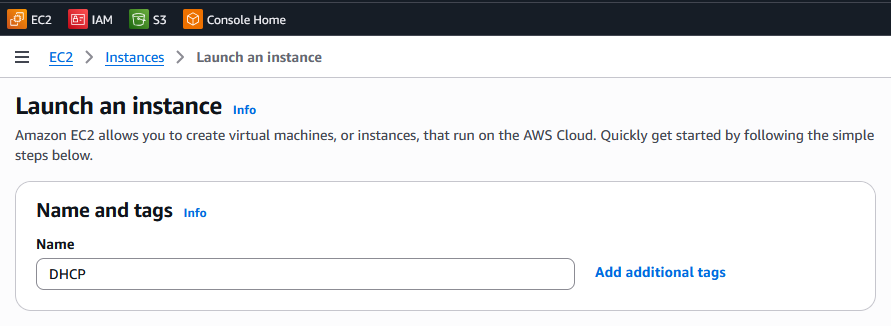
\includegraphics[width=0.9\linewidth]{corps/images/image3}
	%\caption{}
	\label{fig:3}
\end{figure}
\newpage
\subsection{Création de la « key pair »}
\begin{figure}[h!]
	\centering
	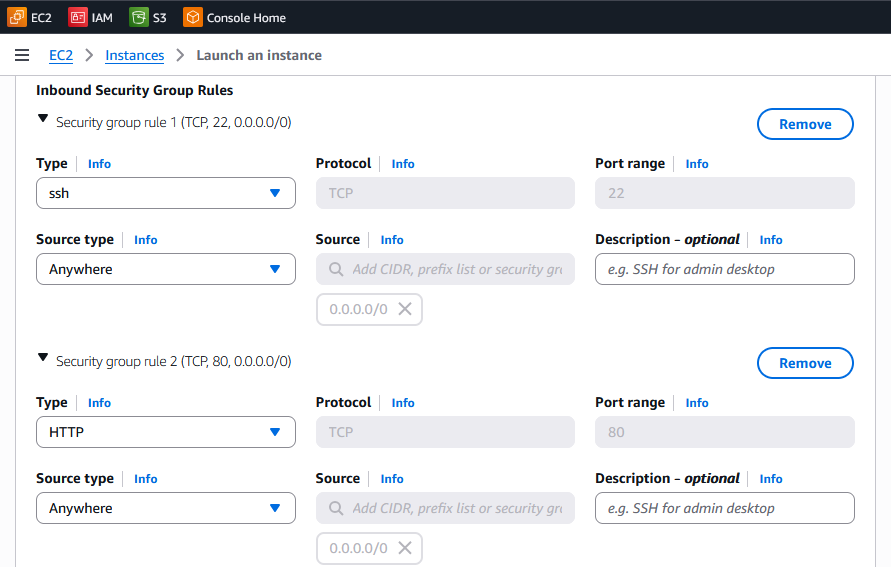
\includegraphics[width=0.7\linewidth]{corps/images/image4}
	%\caption{}
	\label{fig:4}
\end{figure}

\subsection{Paramétrage du réseau de l’instance}
\begin{figure}[h!]
	\centering
	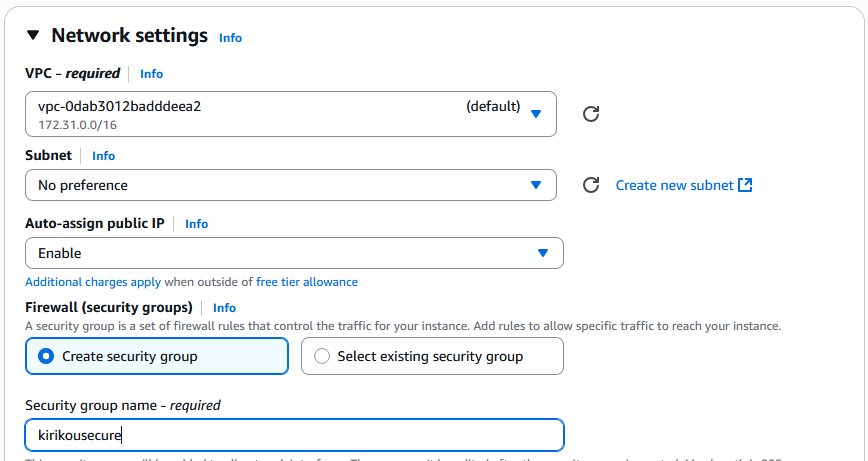
\includegraphics[width=0.8\linewidth]{corps/images/image5}
	%\caption{}
	\label{fig:5}
\end{figure}
\newpage
\subsection{Définition des règles du groupe de sécurité pour l’accès à l’instance}
\begin{figure}[h!]
	\centering
	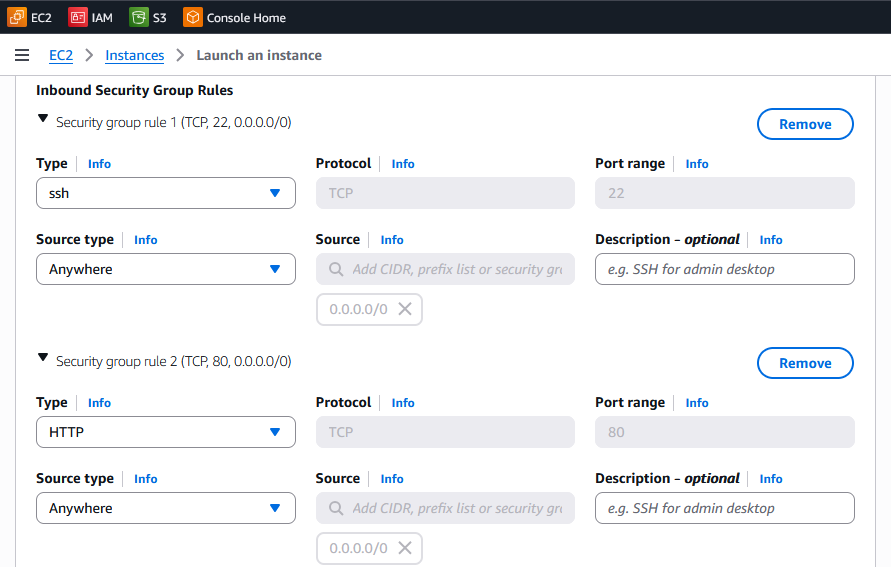
\includegraphics[width=0.7\linewidth]{corps/images/image6}
	%\caption{}
	\label{fig:6}
\end{figure}

\subsection{Configuration du stockage de l’instance}
\begin{figure}[h!]
	\centering
	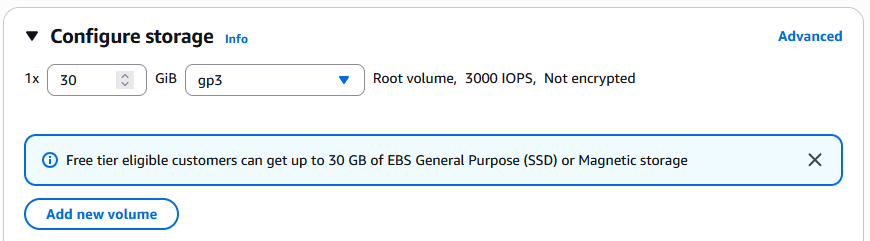
\includegraphics[width=0.9\linewidth]{corps/images/image7}
	%\caption{}
	\label{fig:7}
\end{figure}
\newpage
\subsection{Récapitulatif de l'instance avant lancement}
\begin{figure}[h!]
	\centering
	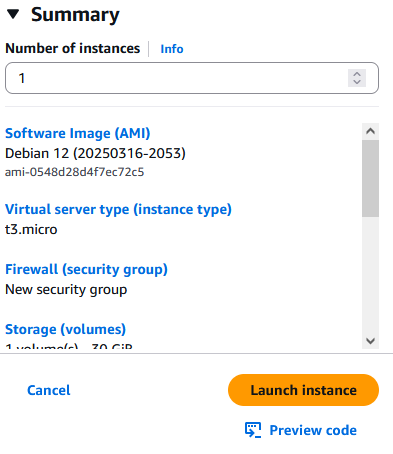
\includegraphics[width=0.6\linewidth]{corps/images/image8}
	%\caption{}
	\label{fig:8}
\end{figure}

\subsection{Connexion à distance avec SSH pour accéder à l’instance EC2}
\begin{figure}[h!]
	\centering
	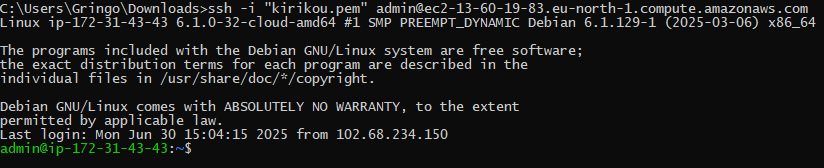
\includegraphics[width=1\linewidth]{corps/images/image9}
	%\caption{}
	\label{fig:9}
\end{figure}

\subsection{Connexion à distance via SSH}
La connexion à distance à l'instance EC2 a été réalisée avec succès. On observe que la session s’est ouverte correctement sur l’instance, ce qui confirme les éléments suivants :

\begin{itemize}
	\item Le groupe de sécurité AWS autorise bien les connexions entrantes sur le port \textbf{22} (SSH).
	\item La clé \texttt{SSH} a été correctement associée à l’instance EC2.
	\item L’instance est fonctionnelle et prête à recevoir les prochaines configurations (serveur DHCP, pare-feu, etc.).
\end{itemize}

\subsection*{Commande utilisée pour le transfert du script}

Le script a été transféré de la machine locale vers l’instance EC2 à l’aide de la commande suivante :

\begin{lstlisting}
	scp -i "C:\Users\Gringo\Downloads\kirikou.pem" \
	"C:\Users\Gringo\Downloads\Mini\script_dhcp_docker_firewall.sh" \
	admin@ec2-13-60-19-83.eu-north-1.compute.amazonaws.com:/home/admin/
\end{lstlisting}

\subsection*{Résolution du problème d'encodage sur Debian}

Sur certaines distributions Debian, le script peut contenir des caractères invisibles (carriage return $ `^M` $) si créé sous Windows. Voici la solution appliquée pour corriger ce problème :

\begin{lstlisting}[language=bash]
	sudo apt update
	sudo apt install dos2unix
	dos2unix script_dhcp_docker_firewall.sh
\end{lstlisting}

\subsection*{Exécution du script sur l’instance}

Avant exécution, le script a été rendu exécutable puis lancé :

\begin{lstlisting}[language=bash]
	chmod +x script_dhcp_docker_firewall.sh
	./script_dhcp_docker_firewall.sh
\end{lstlisting}

\begin{figure}[h!]
	\centering
	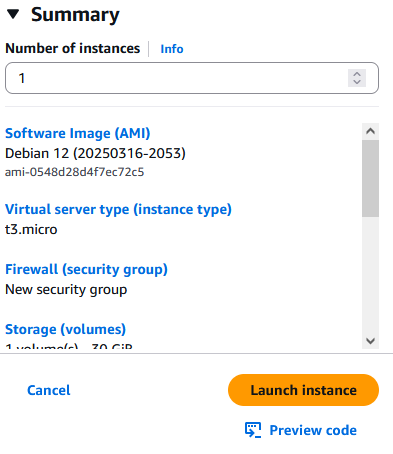
\includegraphics[width=1\linewidth]{corps/images/image10}
	%\caption{}
	\label{fig:10}
\end{figure}
\begin{center}
	Image d’installation de l’image Docker
\end{center}
\section{Conclusion}
	Ce projet montre la capacité à automatiser le déploiement d’un service réseau (DHCP) dans un conteneur sécurisé via Docker. Le script facilite la configuration dynamique et renforce la sécurité grâce à iptables. Cette approche est généralisable à d’autres services dans une infrastructure DevOps moderne.
\newpage	
\section*{Références}
	\begin{itemize}
		\item {https://docs.docker.com/engine/install/debian/}
		\item {https://www.hostinger.fr/tutoriels/iptables}
		\item {https://www.it-connect.fr/serveur-dhcp-sous-linux/}
		\item {https://www.it-connect.fr/installation-pas-a-pas-de-docker-sur-debian-11/}
	\end{itemize}
	\newpage
	\section*{Annexe : Script Bash complet}
	
	\begin{lstlisting}[language=bash]
		#!/bin/bash
		
		set -e
		
		if [ "$EUID" -ne 0 ]; then
		echo "Ce script doit être exécuté avec les droits root. Utilisez 'sudo ./setup-dhcp-firewall.sh'"
		exit 1
		fi
		
		echo "[1/8] Demande des informations de configuration réseau pour le DHCP..."
		read -p "Adresse réseau (ex: 192.168.100.0): " RESEAU
		read -p "Masque de sous-réseau (ex: 255.255.255.0): " NETMASK
		read -p "Adresse IP de début (ex: 192.168.100.100): " IP_DEBUT
		read -p "Adresse IP de fin (ex: 192.168.100.200): " IP_FIN
		read -p "Passerelle (ex: 192.168.100.1): " GATEWAY
		read -p "DNS (ex: 8.8.8.8): " DNS
		
		echo "[2/8] Mise à jour du système et installation de Docker..."
		apt update && apt upgrade -y
		apt install -y ca-certificates curl gnupg lsb-release
		
		install -m 0755 -d /etc/apt/keyrings
		curl -fsSL https://download.docker.com/linux/debian/gpg -o /etc/apt/keyrings/docker.asc
		chmod a+r /etc/apt/keyrings/docker.asc
		
		echo "deb [arch=$(dpkg --print-architecture) signed-by=/etc/apt/keyrings/docker.asc] https://download.docker.com/linux/debian $(. /etc/os-release && echo \"$VERSION_CODENAME\") stable" | tee /etc/apt/sources.list.d/docker.list > /dev/null
		
		apt update
		apt install -y docker-ce docker-ce-cli containerd.io docker-buildx-plugin docker-compose-plugin
		
		echo "[3/8] Nettoyage des anciens fichiers (si présents)..."
		rm -rf docker-firewall
		docker rm -f mon-serveur-dhcp 2>/dev/null || true
		docker image rm dhcp-firewall 2>/dev/null || true
		
		echo "[4/8] Création des fichiers Docker..."
		mkdir -p docker-firewall
		cd docker-firewall
		
		# script-firewall.sh
		cat > script-firewall.sh << 'EOF'
		#!/bin/bash
		iptables -F
		iptables -X
		iptables -P INPUT DROP
		iptables -P FORWARD DROP
		iptables -P OUTPUT ACCEPT
		iptables -A INPUT -i lo -j ACCEPT
		iptables -A INPUT -m conntrack --ctstate ESTABLISHED,RELATED -j ACCEPT
		iptables -A INPUT -p icmp --icmp-type 8 -j DROP
		netfilter-persistent save
		EOF
		
		# script-dhcp.sh
		cat > script-dhcp.sh << EOF
		#!/bin/bash
		echo 'DHCPDv4_CONF=/etc/dhcp/dhcpd.conf' > /etc/default/isc-dhcp-server
		echo 'INTERFACESv4="enp0s3"' >> /etc/default/isc-dhcp-server
		
		cat <<EOL > /etc/dhcp/dhcpd.conf
		option domain-name "gerioux.com";
		default-lease-time 345600;
		max-lease-time 691200;
		authoritative;
		log-facility local7;
		
		subnet $RESEAU netmask $NETMASK {
			range $IP_DEBUT $IP_FIN;
			option domain-name-servers $DNS;
			option routers $GATEWAY;
		}
		EOL
		
		systemctl restart isc-dhcp-server.service
		EOF
		
		# Dockerfile
		cat > Dockerfile << 'EOF'
		FROM debian:stable-slim
		
		RUN apt update && apt install -y iptables iptables-persistent isc-dhcp-server net-tools nano systemctl
		
		COPY script-dhcp.sh /root/script-dhcp.sh
		COPY script-firewall.sh /root/script-firewall.sh
		
		RUN chmod +x /root/script-dhcp.sh /root/script-firewall.sh
		
		CMD /root/script-firewall.sh && /root/script-dhcp.sh && tail -f /dev/null
		EOF
		
		chmod +x script-dhcp.sh script-firewall.sh
		
		echo "[5/8] Construction de l’image Docker..."
		docker build -t dhcp-firewall .
		
		echo "[6/8] Lancement du conteneur DHCP + Pare-feu..."
		docker run --rm --net=host --cap-add=NET_ADMIN --name mon-serveur-dhcp dhcp-firewall
	\end{lstlisting}
	
